\chapter{Software Implementierung}

\section{PX4} \label{px4:subsection}
PX 4 ist eine Open-Source-Software, welche zur Steuerung verschiedener Arten von Fahrzeugen genutzt werden kann, hierzu zählen beispielsweise verschiedene Drohnenarten, sowie auch Fahrzeuge auf dem Boden und Unterwasserfahrzeuge.\\ Es kann zum einen für bereits flugfähigen Drohen eingesetzt werden. Aber es besteht auch die Möglichkeit eine neue Drohne in Verbindung mit PX4 zu bauen.\\
Für die Verwendung der PX4 Software kann QGroundControl (siehe Kapitel \ref{qGroundControl:subsection}) verwendet werden. \cite[vgl.][]{px4} \\
Der PX4-Flugstack wurde ursprünglich nur dür die Pixhawk-Hardware entwickelt, allerdings ist es heutzutage auch möglich diesen auf Linux-Computern und anderen Hardware einzusetzen. Wie es auch bei der Coex Clover Drohne mit dem Coex Pix umgesetzt wird. \\
Die Software setzt Sensoren, ein um den Zustand der Drohne zu bestimmen. Hierfür werden einige Sensoren vorausgesetzt, zu diesen zählen ein Gyroskop, ein Beschleunigungssensor, ein Magnetometer sowie ein Barometer. Zudem ist GPS empfohlen um weitere Modi nutzen zu können. \cite[vgl.][]{px4}

\subsection{Flugmodi}
PX4 bietet verschiedene Flugmodi an, welche das Verhalten der des jeweiligen Fahrzeuge beziehungsweise Drohnen steuert und auch regelt, wie jeweils auf Benutzereingaben regiert werden soll. Das Wechseln dieser Flugmodi kann zum einen über die QGroundControl Software (siehe Kapitel \ref{qGroundControl:subsection}) oder auch je nach Anpassung der Fernbedinung, beispielsweise über verschiedene Schalter, auf dieser vollzogen werden. \\
Allerdings muss auch beachtet werden, dass nicht alle Flugmodi bei allen Drohnen oder Fahrzeugen einsetzbar sind. Aussschlaggebend hierfür ist vor allem die Ausstattung des. Da jeder Flugmodi bestimmte Bedingungen hat die erfüllt sein müssen, beispielsweise Sensoren wie ein Geschwindikgeitssensor. \\
Die Flugmodi lassen sich in drei Kategorien einteilen, diese sind manuelle, ünterstütze sowie automatische Steuerung.
Da es bei diesem Projekt um den Einsatz einer Drohne handelt, werden im folgenden lediglich die für Drohnen relevanten Flugmodi erläutert.
Zu der manuellen Steuerung, bei welchem der Pilot die Drohne direkt und ohne direkte UNterstützung steuert, gehören unter anderem die Modi "manuell" beziehungsweise "stabilisiert". Diese sorgen für eine stabilisierte horizontale Ausrichtung, jedoch ermöglichen sie es dem Piloten hierbei, das Gaspedal sowie die Roll- und Neigbewegungen selbst zu bestimmen. Zu dieser Katergorie gibt es noch weitere Modi, welche allerdingsa hauptsächlich für Flugshows genutzt werden.
Bei der unterstützen Steuerung kann aus zwei verschiedenen Flugmodi gewählt werden, "ALTCTL (Altitude)" und "POSCTL (Position)". Beim ALTCTL-Modi wird besonders die Höhe der Drohne von Autopliot gesteurt, sodass diese einen möglichst konstanten Abstand zum Boden hält. Dieser Modi benötigt hierfür ein Barometer oder andere Sensoren zur Höhenmessung.
Der POSCTL dient zum Halten der Position der Drohne, das heißt neben der Höhe werden zudem die Bewegungsgeschwindkeit nach vorne, hinten und zur Seite gesteuert, um die Drohne möglichst auf einer bestimmten Position zu halten.\\
Bei der automatischen Steuerung fliegt die Drohne automatische ohne Benutzereingaben mittels eines Programms. Zu dieser Katergorie gehört der "Offboard"-Modus hierdurch ist es möglich, dass die Drohne durch einen anderen Computer gesteuert werden kann. Zudem gibt es noch einen Missions-Modus, hierbei kann beispielsweise über QGroundControl ein Pfad geplant werden, welcher dann von der Drohne mittels GPS geflogen wird. \\
Für das Projekt ist hierbei vor allem der Offboard-Modus von Bedeutung, da dieser benötigt wird, um autonome Flüge mit der Coex Clover Drohne zu machen, da diese hierbei von dem Raspberry Pi gesteuert wird. \cite[vgl.][]{flight-modes}


\subsection{QGroundControl}  \label{qGroundControl:subsection}
QGroundControl ist eine Software, welche vor allem für Drohnen mit einem PX4 aber auch anderen Flight Controller genutzt werden kann. Hierbei bietet es verschiedene Funktionen. Zum einen gehört hierzu die Konfiguration der einzelnen  Drohnen. Desweiteren ist es möglich mit der Software verschiedene Flugmodi auszuwählen, sowie diese dann auch während des Fluges zu überwachen, beispielweise durch die Anzeige der Flugposition auf einer Karte sowie auch deren Geschwindigkeit und andere Sensordaten.
Es ist auch möglich mit QGroundControl eine ganze Flugplanung zu machen, welche die Drohne daraufhin umsetzt. \cite[vgl.][]{qGroundControl}


\section{Systemarchitektur}

\subsection{Allgemeine Systemarchitektur eines ROS Programms}
Das Robot Operating System (ROS) hat den Bereich der Robotik revolutioniert, indem es einen robusten und flexiblen Rahmen für die Entwicklung komplexer Robotersysteme bietet. Das Herzstück von ROS ist seine ausgeklügelte Systemarchitektur, die das Zusammenspiel zwischen verschiedenen Komponenten orchestriert und eine nahtlose Kommunikation und Koordination ermöglicht.

\subsubsection{Zentrale Konzepte}
\begin{description}
    \item[Nodes:] Nodes sind autonome Softwaremodule, die bestimmte Aufgaben innerhalb eines ROS-Systems übernehmen. Sie kommunizieren miteinander, indem sie Nachrichten zu Themen veröffentlichen und abonnieren oder indem sie Services aufrufen und bereitstellen. Nodes können über mehrere Maschinen verteilt sein und bilden so ein verteiltes System.
    
    \item[Topics:] Topics sind benannte Busse, über die Nodes Nachrichten austauschen. Nachrichten werden von einem oder mehreren Nodes in Topics veröffentlicht und von Nodes abonniert, die am Empfang der Daten interessiert sind. Topics verwenden ein Publish-Subscribe-Messaging-Muster, das eine asynchrone Kommunikation ermöglicht und die Sender- und Empfängernodes entkoppelt.
    
    \item[Messages:] Nachrichten sind die Datenstrukturen, die für die Kommunikation zwischen Nodes verwendet werden. Sie werden in ROS mithilfe der Interface-Definition Language (IDL) oder Nachrichtenbeschreibungsdateien (.msg) definiert. Nachrichten können einfach sein, z. B. numerische Werte oder Zeichenketten, oder komplex, bestehend aus verschachtelten Strukturen und Arrays.
    
    \item[Services:] Services ermöglichen eine synchrone Anfrage-Antwort-Kommunikation zwischen Nodes. Ein Node bietet einen Service an, und andere Node können Anfragen an ihn senden. Die Dienstnode verarbeitet dann die Anforderung und sendet eine Antwort an den anfordernden Node zurück. Services werden mithilfe von .srv-Dateien definiert und folgen einem Client-Server-Kommunikationsmuster.
\end{description}

\subsubsection{Schichten der ROS-Systemarchitektur}
\begin{description}
    \item[Dateisystem-Ebene:] Die Dateisystem-Ebene in \ac{ROS} spielt eine entscheidende Rolle bei der Organisation und Verwaltung der für die Entwicklung von Roboteranwendungen erforderlichen Ressourcen. Sie bietet eine hierarchische Struktur und Paketverwaltungsfunktionen, die es Entwicklern ermöglichen, ihren Code, ihre Konfigurationsdateien, Startdateien und Daten effizient zu organisieren. Die \ac{ROS} Filesystem-Ebene dient als Grundlage für den Aufbau modularer und wiederverwendbarer Softwarekomponenten innerhalb des \ac{ROS}-Ökosystems.

    Der Kern der \ac{ROS} Filesystem-Ebene ist das Konzept der Pakete. Ein Paket in \ac{ROS} ist eine Verzeichnisstruktur, die eine Sammlung zusammengehöriger Dateien enthält, einschließlich Code, Konfigurationsdateien und Datenressourcen. Pakete bieten einen modularen Ansatz zur Organisation von Code und erleichtern die Wiederverwendung von Code über verschiedene Projekte hinweg. Sie kapseln eine bestimmte Funktionalität oder ein Merkmal und können unabhängig entwickelt, getestet und verteilt werden.
    
    Die \ac{ROS}-Dateisystem-Ebene folgt einem auf Konventionen basierenden Ansatz für die Organisation von Paketen. Ein typisches \ac{ROS}-Paket enthält eine Manifestdatei namens package.xml, die Metadaten und Abhängigkeiten für das Paket enthält. Darüber hinaus folgt die Verzeichnisstruktur des Pakets einem bestimmten Layout, mit Verzeichnissen wie src für Quellcode, launch für Startdateien, msg für Nachrichten-Definitionsdateien und config für Konfigurationsdateien. Diese einheitliche Struktur verbessert die Zusammenarbeit und ermöglicht es den Entwicklern, Ressourcen innerhalb eines Pakets leicht zu finden und darauf zuzugreifen.
    
    Die Paketverwaltungswerkzeuge in \ac{ROS} bieten wichtige Funktionen für die Verwaltung von Paketen. Das Werkzeug rospack ermöglicht es Benutzern, Pakete im Dateisystem zu finden und Informationen über ihre Abhängigkeiten abzurufen. Es hilft beim Auffinden von Paketpfaden, beim Abrufen von Paket-Metadaten und beim Auflösen von Paketabhängigkeiten. Das Werkzeug rosdep kümmert sich um die Installation von Paketabhängigkeiten, indem es automatisch die von \ac{ROS}-Paketen benötigten Abhängigkeiten auf Systemebene auflöst und installiert.
    
    Darüber hinaus unterhält die \ac{ROS}-Community ein zentrales Paket-Repository, den \ac{ROS} Package Index (https://index.ros.org/packages/). Der \ac{ROS} Package Index ist eine umfassende Sammlung von \ac{ROS}-Paketen, die von Entwicklern weltweit zur Verfügung gestellt werden. Er dient als wertvolle Ressource für die Entdeckung und den Austausch von Paketen und fördert die Zusammenarbeit und die Wiederverwendung von Code innerhalb des \ac{ROS}-Ökosystems.
    
    \item[Berechnungsgraphen-Schicht:] Die Berechnungsgraphenschicht ist das Rückgrat von ROS und verwaltet die Interaktionen zwischen den Nodes. Sie visualisiert die Beziehungen zwischen Nodes, Topics und Services in Form eines gerichteten Graphen und ermöglicht so ein klares Verständnis der Systemarchitektur. Der Graph erleichtert die Weitergabe von Nachrichten, die Synchronisation und die Koordination zwischen den Nodes.
    
    \item[Kommunikationsschicht:] ROS verwendet Middleware, wie z. B. die Robot Communication Middleware (RCM) oder FastRTPS, um Kommunikationsdetails auf niedriger Ebene zu behandeln. Die Kommunikationsschicht kümmert sich um die Serialisierung von Nachrichten, Transportprotokolle und Netzwerkkommunikation und abstrahiert diese Komplexitäten vom Entwickler. Diese Schicht gewährleistet eine zuverlässige und effiziente Kommunikation zwischen den Nodes.
    
    \item[Schicht der Client-Bibliotheken:] ROS bietet Client-Bibliotheken in mehreren Programmiersprachen, darunter C++, Python und andere. Diese Bibliotheken bieten High-Level-Abstraktionen und APIs für Entwickler, um ROS-Nodes zu schreiben und mit dem System zu interagieren. Die Client-Bibliotheken vereinfachen den Entwicklungsprozess, indem sie gebrauchsfertige Funktionen zum Erstellen von Nodes, zum Veröffentlichen und Abonnieren von Topics und zum Aufrufen von Services bereitstellen.
    
    \item[Tools-Schicht:] ROS bietet eine Vielzahl von Werkzeugen, die bei der Entwicklung, Fehlersuche und Analyse von ROS-Programmen helfen. Tools wie RViz bieten 3D-Visualisierungsfunktionen, mit denen Entwickler den Zustand und die Umgebung des Roboters visualisieren können. Andere Tools wie rosbag ermöglichen die Aufzeichnung und Wiedergabe von Nachrichtendaten zur Offline-Analyse und Fehlersuche. Die Werkzeugebene steigert die Produktivität und erleichtert eine umfassende Systemanalyse.
    
    \item[Betriebssystem-Schicht:] Die Betriebssystemschicht stellt die zugrundeliegende Infrastruktur bereit, die für den Betrieb von ROS notwendig ist, einschließlich Hardwareabstraktion, Gerätetreiber und Prozessmanagement. ROS ist mit verschiedenen Betriebssystemen wie Linux, macOS und Windows kompatibel und gewährleistet so die Portabilität über verschiedene Plattformen hinweg.
\end{description}

\subsubsection{Schlüsselkomponenten}
\begin{description}
    \item[ROS-Master:] Der ROS-Master ist ein zentraler Benennungs- und Registrierungsdienst, der die Erkennung von Nodes und die Weitergabe von Nachrichten erleichtert. Er verfolgt aktive Nodes, verwaltet Themen- und Dienstregistrierungen und hilft beim Aufbau von Verbindungen zwischen Herausgebern und Abonnenten.
    
    \item[Launch-System:] Das Launch-System ermöglicht es Benutzern, die Launchdateien zu definieren und zu verwalten, die die Konfigurations- und Startparameter für den Betrieb eines ROS-Systems festlegen. Launchdateien erleichtern das Starten mehrerer Nodes mit ihren jeweiligen Parametern und vereinfachen den Initialisierungsprozess.
    
    \item[Parameter-Server:] Der Parameter-Server ist ein verteilter Key-Value-Speicher, der es den Nodes ermöglicht, Parameter gemeinsam zu nutzen und dynamisch darauf zuzugreifen. Die Nodes können Konfigurationsparameter, Kalibrierungswerte oder andere gemeinsam genutzte Daten auf dem Parameter-Server speichern, wodurch sich das Systemverhalten zur Laufzeit leicht konfigurieren und ändern lässt.
    
    \item[ROS-Bags:] ROS-Bags ermöglichen die Aufzeichnung und Wiedergabe von Nachrichten und bieten einen praktischen Mechanismus für Datenprotokollierung, Fehlersuche und Analyse. Entwickler können Nachrichtenströme aufzeichnen und in einer Bag-Datei speichern, die später zur Offline-Analyse wiedergegeben oder zur Simulation von Eingaben während des Testens verwendet werden kann.
\end{description}

\section{Softwarearchitektur}
\todo{Beschreibung Mavros}

    %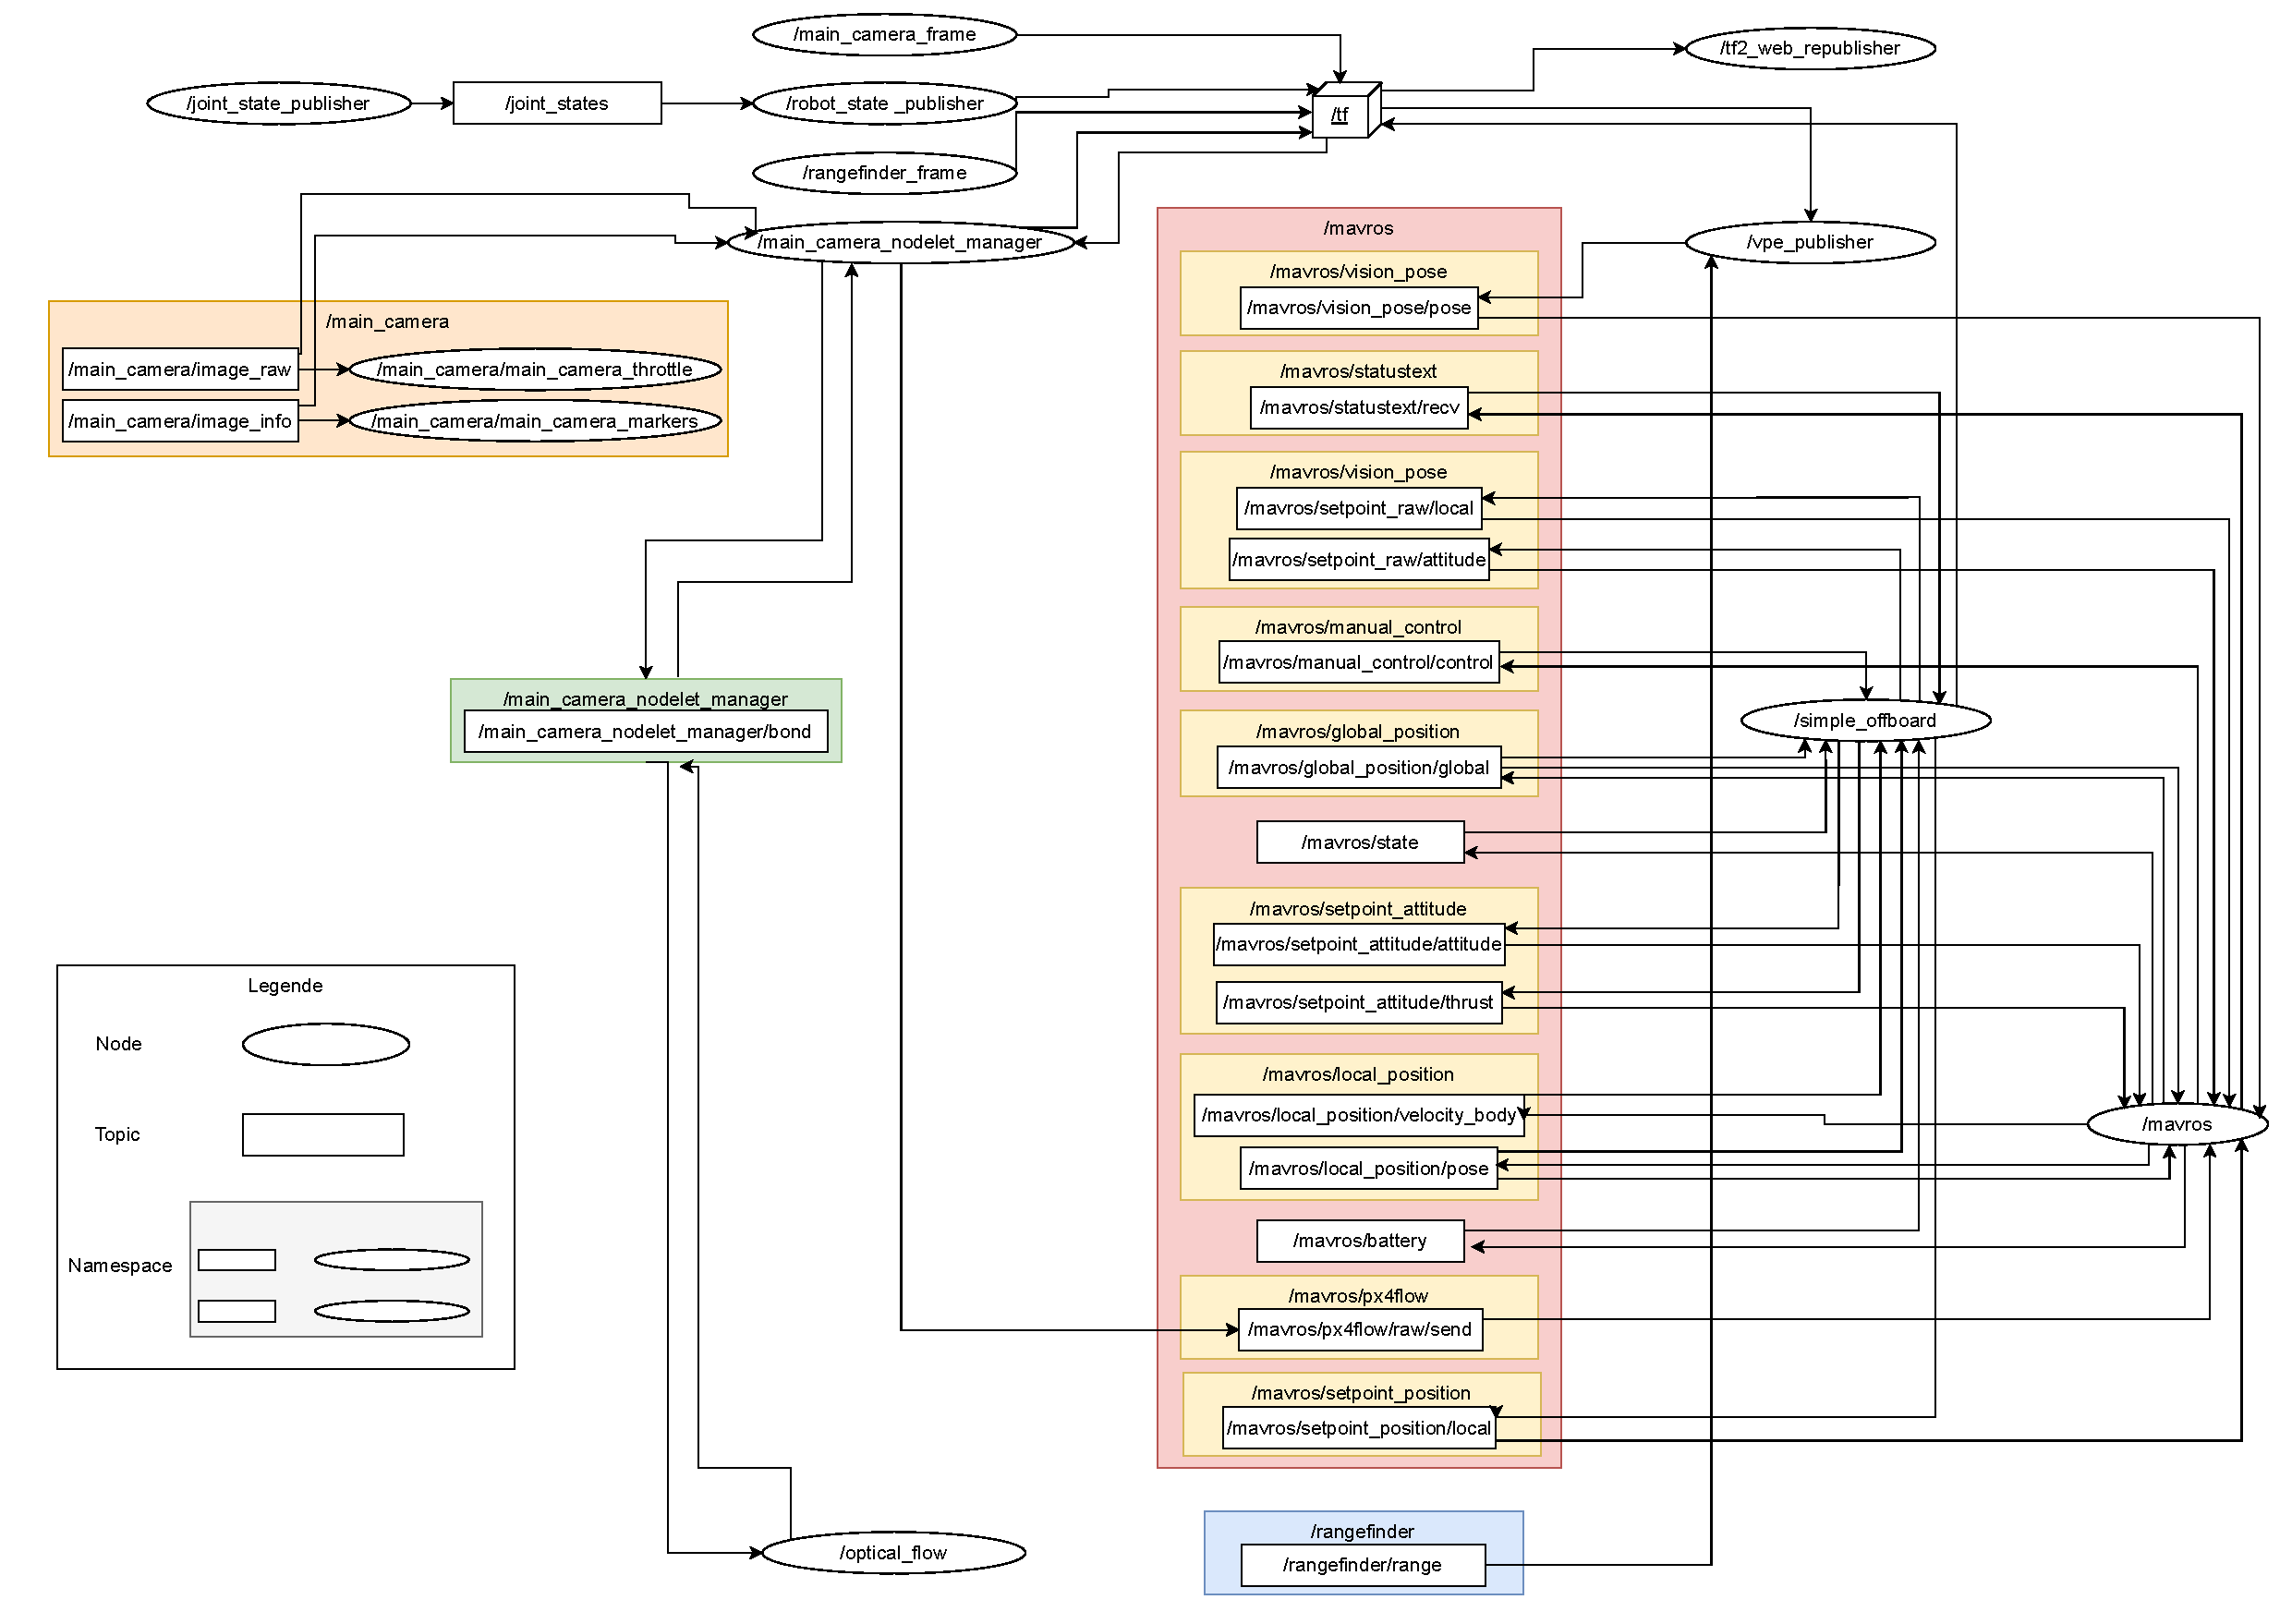
\includepdf[landscape=true]{images/graph_ros.pdf}
    %\caption[Übersicht ROS Nodes]{\label{img ros_nodes_graph} Übersicht ROS Nodes [eigene Darstellung]}
    \begin{landscape}
        \begin{figure}
            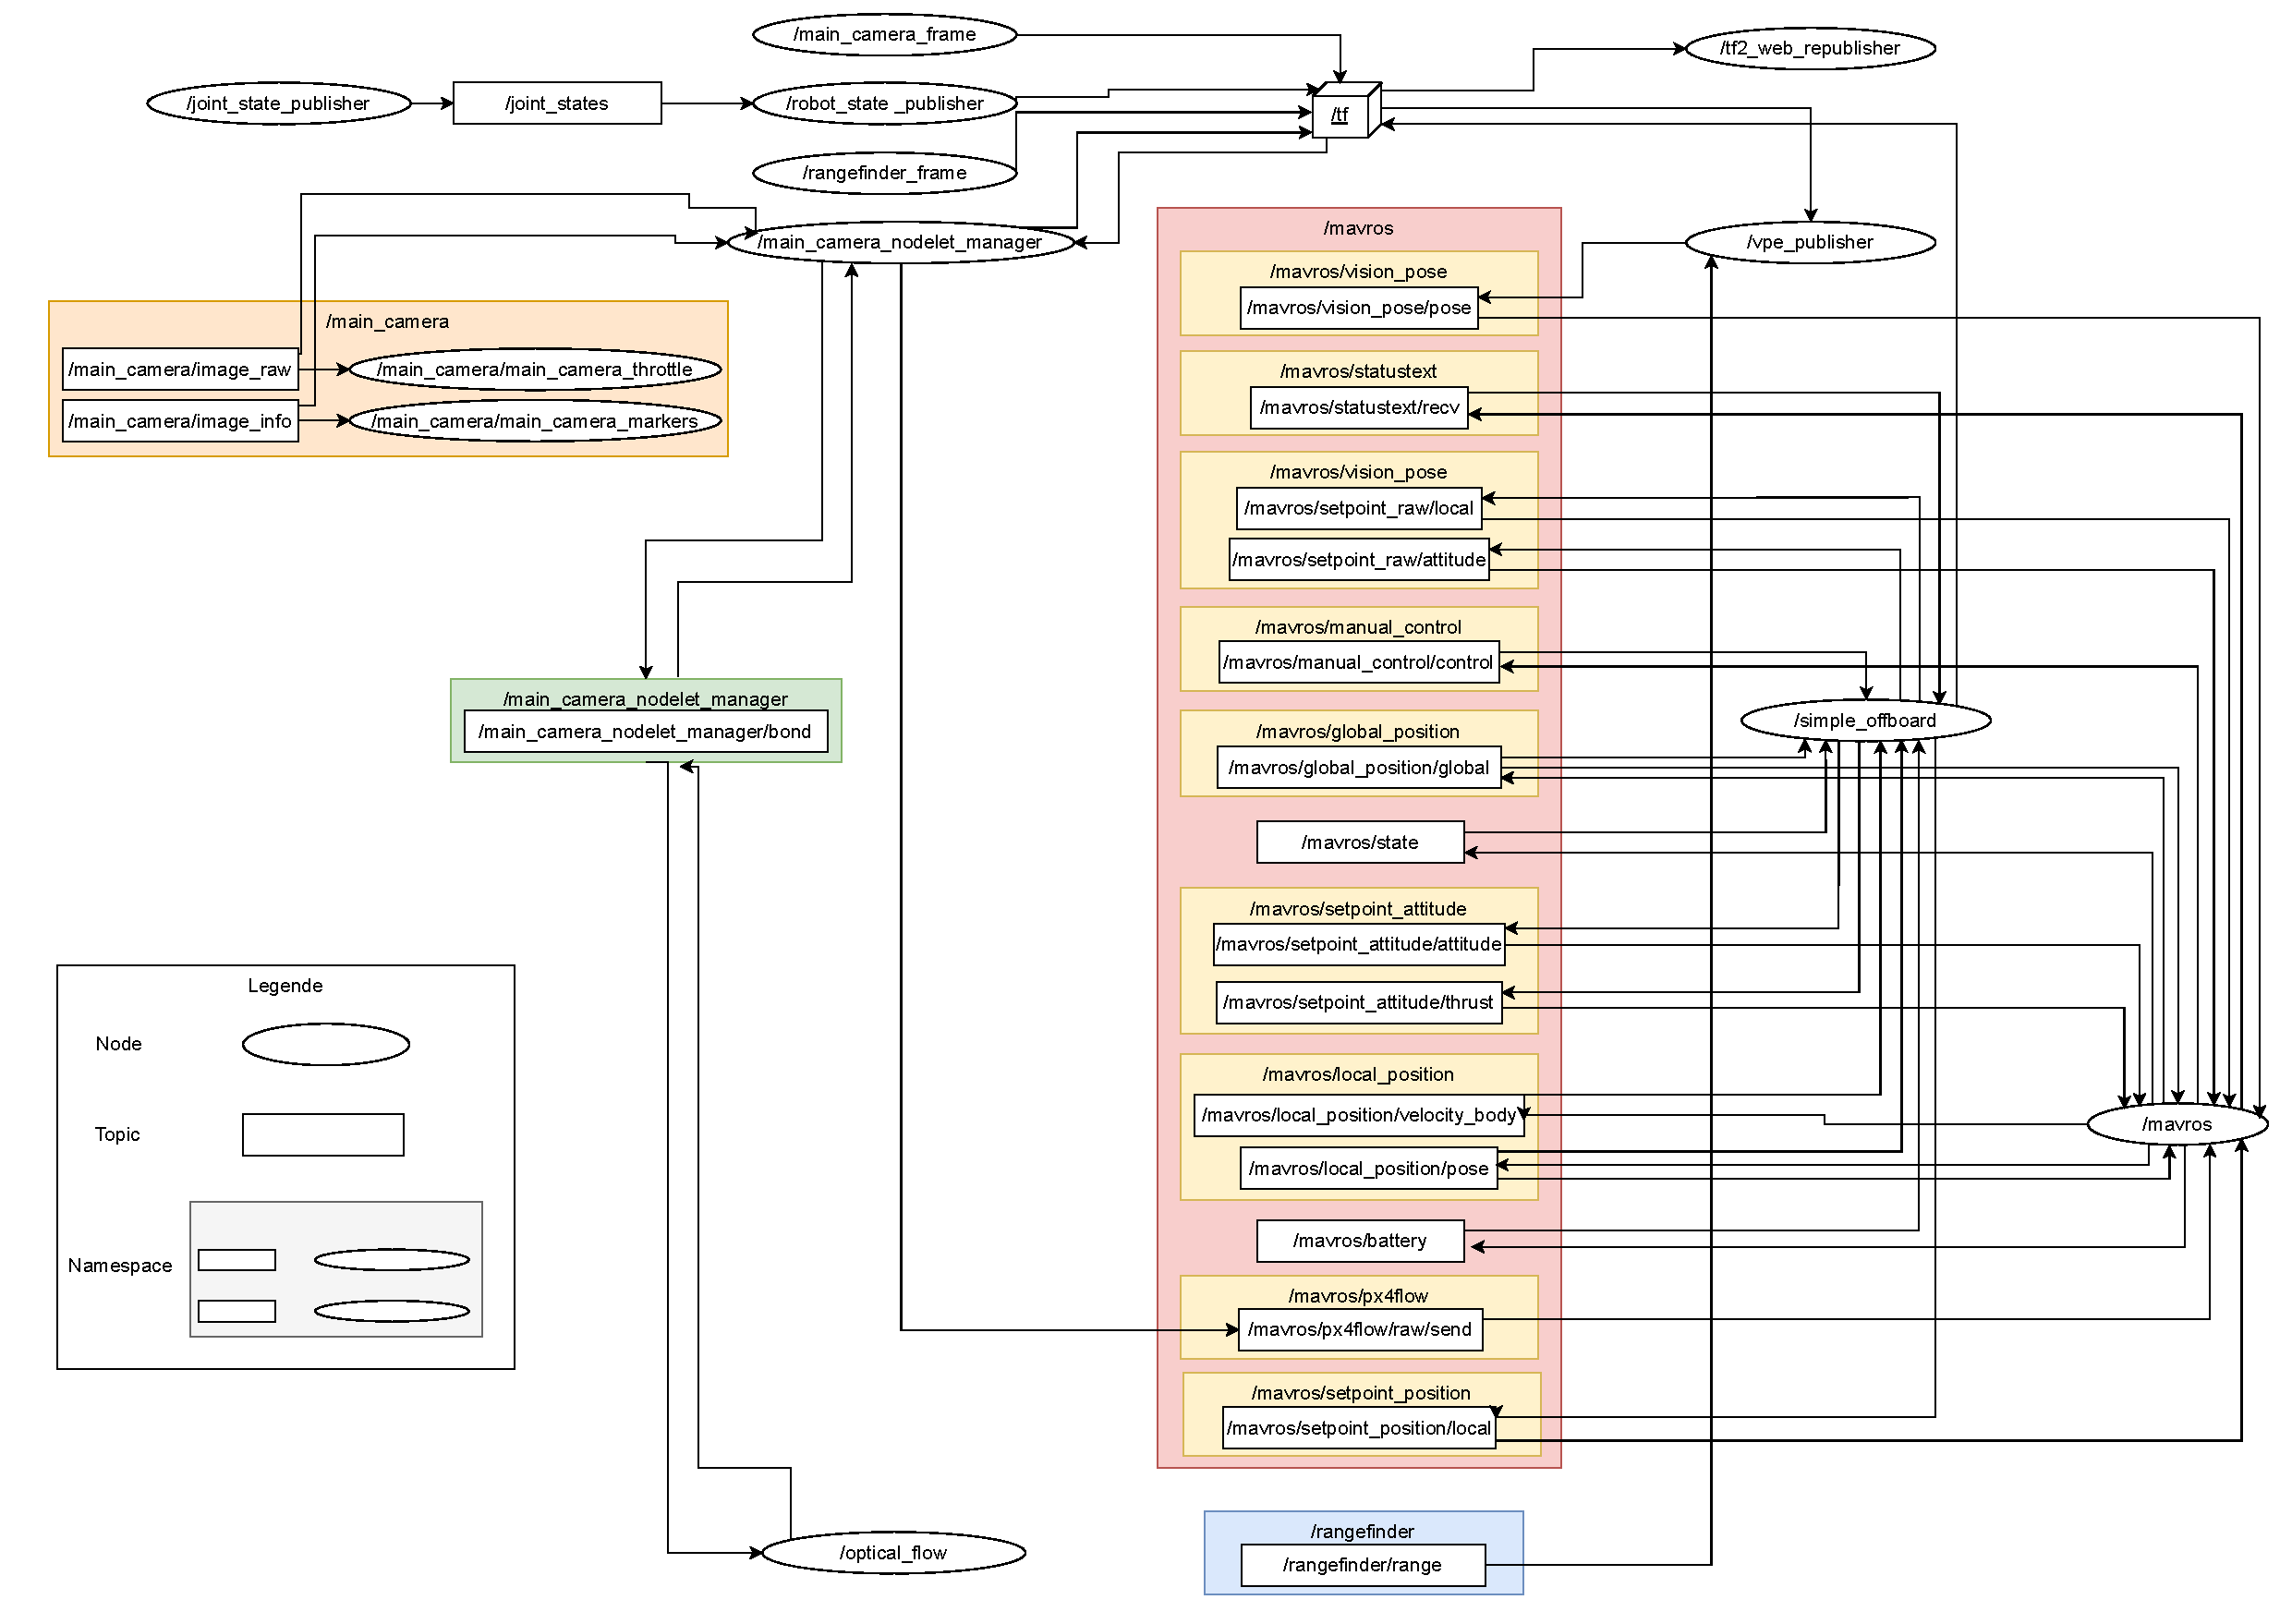
\includegraphics[width=\paperwidth,keepaspectratio]{images/graph_ros.pdf}
            \caption[Übersicht ROS Kommunikation]{\label{img ros_communication} Übersicht ROS Kommunikation [eigene Darstellung]}
        \end{figure}
    \end{landscape}

In der Abbildung \ref{img ros_communication} ist eine Übersicht der Kommunikation zwischen den verschiedenen Komponenten in \ac{ROS} zu sehen. \\
Hauptbestandteil sind hierbei vor allem die Nodes der Hauptkamera beziehungsweise der Azure Kinect sowie auch Mavros. \\
Mavros ist hierbei ein ROS-Paket, welches die Kommunikation zwischen dem Raspberry Pi und der Drohne mit Hilfe des MAVLink-Protokolls (siehe Kapitel \ref{mavlink}) ermöglicht. Es unterstützt dabei unter anderem den PX4 Flightstack, welcher in der Coex Clover Drohne vorhanden ist. Die Kommunikation kann hierbei wie bei MAVLink auch über \ac{USB} oder auch über Wifi stattfinden. \\
Im nachfolgenden wird nun genauere auf einzelne Komponenten der ROS Kommunikation (siehe \ref{img ros_communication}) eingegangen. \\

%https://clover.coex.tech/en/mavros.html


\section{Kalibrierung der COEX Drohne}

\section{Drohnen Autopilot}


\section{3D Modell}
Um die Drohne auch in der Simulation unter echten Bedingungen fliegen zu lassen, müssen die realen Gegebenheiten in die Simulation übertragen werden. Um dies zu bewerkstelligen, muss ein 3D-Modell der Räume erstellt werden, in welchen sich die Drohne bewegen soll.
    \subsection{3D Scan}

        \subsubsection{Microsoft HoloLens 2}
        Um ein 3D-Modell des Raumes mit der Microsoft HoloLens 2 zu erstellen, muss man die integrierte Mixed-Reality-Capture-Funktion der HoloLens 2 verwenden.
        
        Die Mixed-Reality-Capture-Funktion der HoloLens 2 ist eine integrierte Funktion, mit der Benutzer die Möglichkeit haben, die Hologramme, die von der HoloLens 2 dargestellt werden, in Echtzeit aufzuzeichnen und zu teilen. Diese Funktion ermöglicht es Benutzern, ihre Augenbewegungen und Handlungen in einer virtuellen Umgebung aufzuzeichnen, um sie mit anderen zu teilen oder für zukünftige Referenz oder Analyse zu speichern. Die Mixed-Reality-Capture-Funktion der HoloLens 2 kann auch für die Erstellung von Immersive-Mixed-Reality-Videoinhalten verwendet werden, indem sie es ermöglicht, virtuelle Hologramme in eine reale Umgebung zu integrieren. Dies kann für verschiedene Anwendungen wie zum Beispiel für die Erstellung von virtuellen Touren, für die Präsentation von Produkten oder für die Unterhaltungsindustrie eingesetzt werden.
        
        \todo{Erstellen des Modells beschreiben}

        Es ist wichtig zu beachten, dass die Qualität des erstellten 3D-Modells von verschiedenen Faktoren abhängt, wie z.B. der Beleuchtung im Raum und der Genauigkeit des Scans. Eine sorgfältige Vorbereitung des Raums und eine langsame, gründliche Durchführung des Scans können dazu beitragen, ein genaueres und detaillierteres 3D-Modell zu erstellen.
        \subsubsection{Azure Kinect \ac{DK}}

    \subsection{3D Modell Vorbereitung}

\section{Navigation}

\section{Simulation}



